\chapter{Math Gallery: Collection 1}

\section{Overview}

\begin{figure}[H]
    \centering
    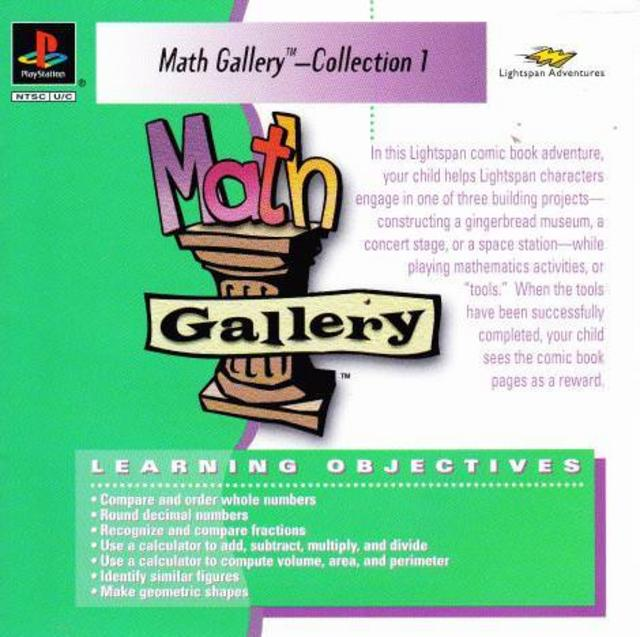
\includegraphics[width=0.5\textwidth]{Games/MathGalleryCollection/Images/MathGalleryCollection1Cover.jpg}
    \caption{Official Math Gallery: Collection 1 CD Cover}
\end{figure}

Math Gallery: Collection 1 features four different types of math for the player to choose from:

\begin{itemize}
    \item Calculaor
    \item Base-10 Blocks
    \item Fraction Strips
    \item Geoboard
\end{itemize}

\section{Transcripts}

\subsection{Series 10}

\subsubsection{Introduction}

Narrator: As our Story begins, Mars Moose arrives in Fairy Tale Island in response to an urgent message he received from his good friend Ginger.

Ginger: Jumpin' jawbreakers! Mars, I'm so glad you're here! Cali and I are overseeing the construction of the Fairy Tale Island Museum, and we need your help.

Mars the Moose: That's my specialty.

Ginger: The weather report calls for a 50\% chance of falling skies this weekend. We need to build the museum and get it glazed as soon as possible.

Mars the Moose: How can I help?

Ginger: I have a construction plan and all of the tools we'll need right here.

\subsubsection{Clip 1}

Mars the Moose: Don't worry Ginger, I'll take care of the landscaping. Whoa, now this is what I call a sticky situation!

\subsubsection{Clip 2}

Pink Animal: How you doing up there, Ginger?

Ginger: This is the last one! I finished the entire roof single-handedly.

\subsubsection{Clip 3}

Ginger: When this frosting hardens, it'll make a beautiful walkway. Right, Mars? Oops!

Pink Animal: Hm, I think it could use just a touch more vanilla.

\subsubsection{Clip 4}

Pink Animal: The gumballs are here!

Mars: Now they're gumdrops!

\subsubsection{Clip 5}

Pink Animal: Wow, the museum is finished, glazed and everything!

Mars the Moose: Cool! Lemon, my favorite!

Ginger: Thanks to your help, Mars! Now all we have to do is collect the items for our exhibits.

Mars the Moose: Hey, I almost forgot! I found this on the way over.

Pink Animal: Cinderella's glass slipper!

Ginger: Leap and lemon drops! This will be the highlight of our famous fairy tale footwear exhibit.

\subsection{Series 20}

Radio Announcer: Next up, the newest hit from K95, the Tail Wag Twist. And don't forget, in the noon hour, we'll be giving away tickets for their sold-out concert this weekend.

Large Brown Dog: Hey Daphne, how's it going?

Daphne: Howlin' Hounds! Good thing you guys are here, we're behind schedule.

Small Grey Dog (Gershwin): Our sound check is scheduled for 4 o'clock. We've got to rehearse the big debut of our new song, "Everything Adds Up."

Large Grey Dog: Hey, we can help! Lend a hand to speed things up!

Female Dog (Ella): Ew, cool! According to Matamozell Magazine, the construction look is in.

Daphne: Well, I have the stage construction plan and all of the tools we'll need right here.

\subsubsection{Clip 1}

Small Grey Dog (Gershwin): We are the dogs who saw and drilled, we like to build because it's such a thrill.

Large Grey Dog: Way to hammer out a new hit song, Gershwin!

\subsubsection{Clip 2}

Large Grey Dog: Hey Ella, what cities have you booked for the rest of our big tour?

Female Dog (Ella): [Los Angeles] and Saint Bernardino.

Large Grey Dog: Woo hoo! California here I come! Ha ha!

\subsubsection{Clip 3}

Small Grey Dog (Gershwin): Maxine do you know which warm-up fans are playing tonight?

Female Dog (Maxine): Three of my absolute favorites: Bowston, The Faux Pas and Electric Howl!

\subsubsection{Clip 4}

Female Dog (Maxine): Hey guys what do you think?

Large Grey Dog: That's one cool look Maxine!

\subsubsection{Clip 5}

Daphne: It's exactly four o'clock. Thanks to your help, the stage is complete just in time for your rehearsal.

Female Dog (Ella): Is everyone ready?

Large Brown Dog: We're ready to go, so let's put on a show!

Female Dog (Maxine): A one, a two, a one, two, two, three, four!

Male Dogs (Singing): Words are floating through my mind every minute of the day. Melodies and harmonies sing out but I wanna say. Now everything adds up, yes everything adds up. Every song that I prepared to conveys the dreams I love to share.

Female Dog (Maxine): Whoa hold up! I broke a drumstick!

Daphne: Tremendous! That's gonna be one of your biggest hits ever!

Large Brown Dog: Hey, what more can you say? Everything adds up!

\subsection{Series 30}

\subsubsection{Introduction}

Narrator: We join our heroes Gracie and Ryan as they arrive at the Spaceport construction site off the distant Moon of Calculatia.

Space Port Operator: How fabulously fortuitous! You got here just in time. Construction is behind schedule, and we could really use a helping hand.

Gracie: I'm ready.

Space Port Operator: We must hurry! An assiduous assemblance of inspectors will arrive in just two days.

Ryan: What can we do to help?

Space Port Operator: I have a comprehensive construction plan and all the tools we'll need right here.

\subsubsection{Clip 1}

Ryan: Gracie, I think you have a screw loose somewhere.

\subsubsection{Clip 2}

Ryan: Have you tied down those rocket pumps yet Gracie?

Gracie: Yes, but I'm at the end of my rope.

\subsubsection{Clip 3}

Ryan: Make sure you set the brakes before you press the -

Gracie: Woah!

Ryan: Red power button.

\subsubsection{Clip 4}

Ryan: Gracie, I must report to level four. Would you mind washing the dishes?

Gracie: I'll get right on it!

\subsubsection{Clip 5}

Inspector: I see that these panels are firmly attached! I find my job absolutely riveting.

Space Port Operator: Inspector Peabody, did we pass the inspection?

Inspector: 100 percent.

Space Port Operator: Wonderful! Now, thanks to Ryan and Gracie, all we need to do is studiously stock the Spaceport with the necessary supplies.

Ryan: And we can open for business right on schedule.

Space Port Operator: Gracie, did you make the sign?

Gracie: I thought you'd never ask.

\subsection{Base-10 Blocks}

Narrator: This is a base-10 unit. 10 units make a rod. 10 rods make a flat. 10 flats make a cube. One cube breaks into ten flats. One flat breaks into ten rods. One rod breaks into ten units. Now we're back to one unit.

\section{Credits}
Concept by: Margy Hillman, Liz Herrick;
Story written by: Liz Herrick;
Vice President, Product Design: Margy Hillman;
Directory, Interactive Products: Liz Herrick;
Program Manager: Heidi Janzen, Darlene Tschudy;
Lead Content Designers: Janet Clark, Kelly Robinson;
Content Designers: Linda Bussell, Amy Nicholson, Ann Rybowiak, Kimberley Tatman;
Senior Program Manager of Curriculum: Sherri Furqueron;
Lead Curriculum Specialist: Jacqueline Gianola-Quinn;
Curriculum Specialist: Janice Morton, Tim Scheidt;
Editor: Helen Hansen;
Curriculum Consultants: Nicholas Branca Ph.D., Judith Jacobs Ph.D., Teri Perl Ph.D.;
Interactive Game Coordinator: Janene Wittmayer;
Director, Curriculum Design: Judy Carr;
Curriculum Support: Aimée Bachmann, Shelly Crickett;
Writer: John Dorsey;
Desktop Publisher: Dave Mauch;
Vice President, Studio Production: Joanne Odenthal, Ph.D.;
Executive Producer: David Hamby;
Animation Director: Al Lowenheim;
Interactive Producer: David Adams;
Associate Producers: Jennifer Mah Hindman, Jo Anne Palasi;
Production Manager: Janet Dahle;
Director, Media Production Technologies: D. Scott Murdoch;
Assistant Art Director: Ken Anderson;
Unit Manager, Preproduction and 2-D: Jan Hastings;
Assistant Directors: Burt Vincent Julio, Luther McLaurin, Jeff Merghart, Rosemary Rodgers, Virgil Sanico, Stania Vanger;
Unit Manager, Interactive: Eydie Gilley;
Background Artists: Dan Jones, Callie Mack, Edgardo Magsino, Suzy Sadak, Judy Temple;
Graphic Artist: Sean Jackson;
3-D Manager/Senior Compositor: Eric Fuss;
Unit Manager, Post Production and 3-D: Colleen McPhillips;
Audio Producer: Rick Bowman;
Audio Engineers: Brad Aldredge, Chris Jahnkow;
Voice Talent: Eileen Bowman, Deem Bristow, Deanna Driscoll, Deanna Hurst, Ron Jones, Paul James Kruse, Royal Lihzis, Mike Lowe, Lani Minella, Deborah Washington;
Asset Management Supervisor: Monica Chernus;
Production Control Technician: David Martin;
Technical Editors: Sandy Mazur, Lori Silfen;
Data Management Assistant: Sjoukie Cooper-Holt;
Asset Management Archivist: Katharine Laxa;
Executive Administrator: Rae Farley;
Director, Software Development: Sergio Garcia;
Director, Software Technology: William Volk;
Development Manager: Robert Warren;
Lead Software Engineer: Janet Academia;
Software Engineers: Tuan Nguyen, Tina Phan;
Graphic Artist: Joy Schmalfeldt;
Production Assistant: Tonette Salter;
Quality Assurance Manager: Mark Myers;
Quality Assurance Supervisors: Ray Nichols, Fred Pecoroni;
Quality Assurance Analysts: James Cajala, Parish Goynes, Randy Jones, Jenna Payne, Janet Row, Geno Vici, Tony Vo;
Quality Assurance Testers: Coni Anselmi, Kevin Garcia, David Hickson, Barbara King, Richard Kriegler, Bill O'Bannon, Ines Panchenko, Barry Rader, Kristin Rix, Marlan Wilson;

\clearpage
\newpage

\section{Screenshots}

\begin{figure}[H]
    \centering
    \begin{subfigure}{0.45\textwidth}
        \centering
        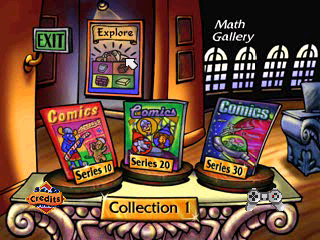
\includegraphics[width=\linewidth]{Games/MathGalleryCollection/Images/MathGalleryCollection1Image1.png}
        \caption{Math Gallery: Collection 1 - Screenshot 1}
    \end{subfigure}
    \begin{subfigure}{0.45\textwidth}
        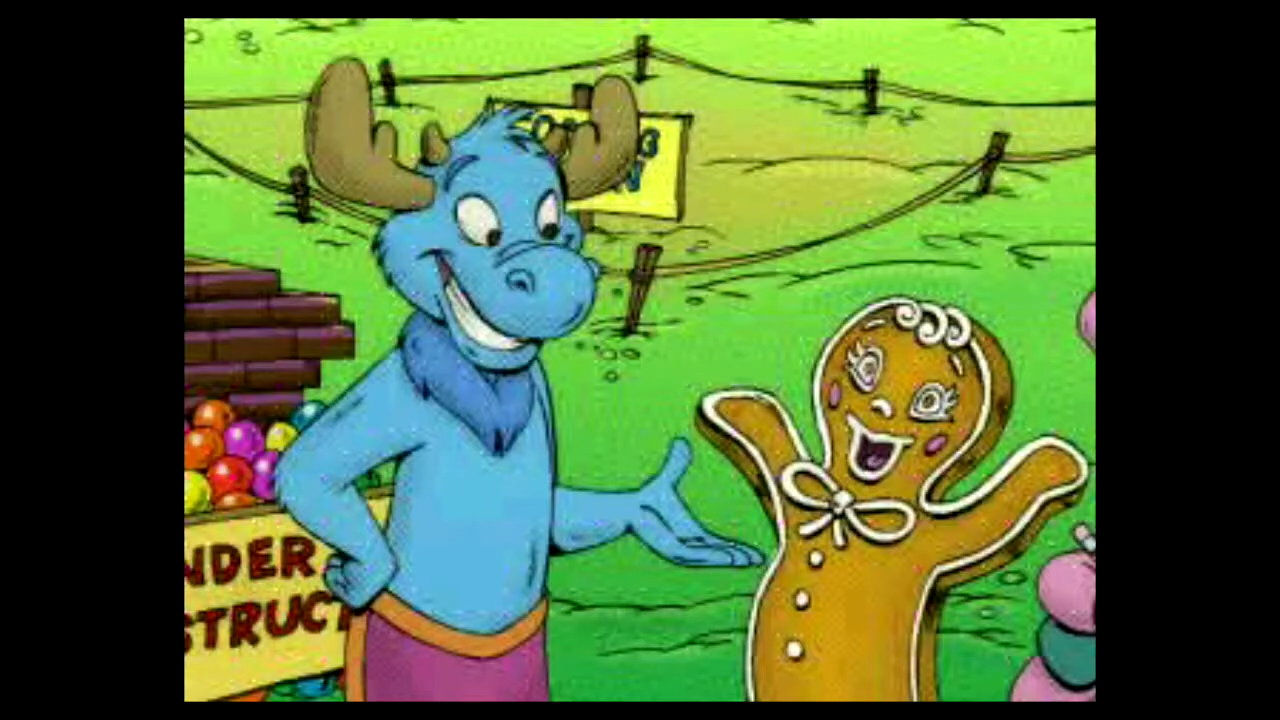
\includegraphics[width=\linewidth]{Games/MathGalleryCollection/Images/MathGalleryCollection1Image2.png}
        \caption{Math Gallery: Collection 1 - Screenshot 2}
    \end{subfigure}

    \begin{subfigure}{0.45\textwidth}
        \centering
        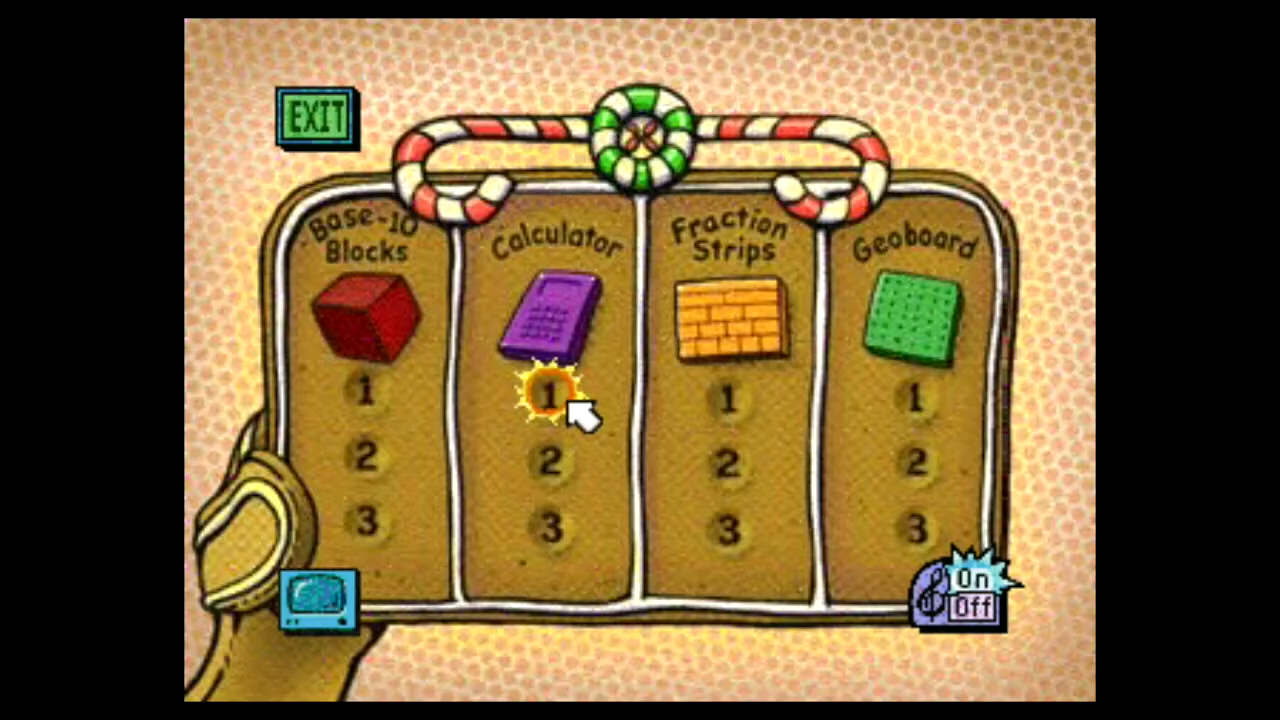
\includegraphics[width=\linewidth]{Games/MathGalleryCollection/Images/MathGalleryCollection1Image3.png}
        \caption{Math Gallery: Collection 1 - Screenshot 3}
    \end{subfigure}
    \begin{subfigure}{0.45\textwidth}
        \centering
        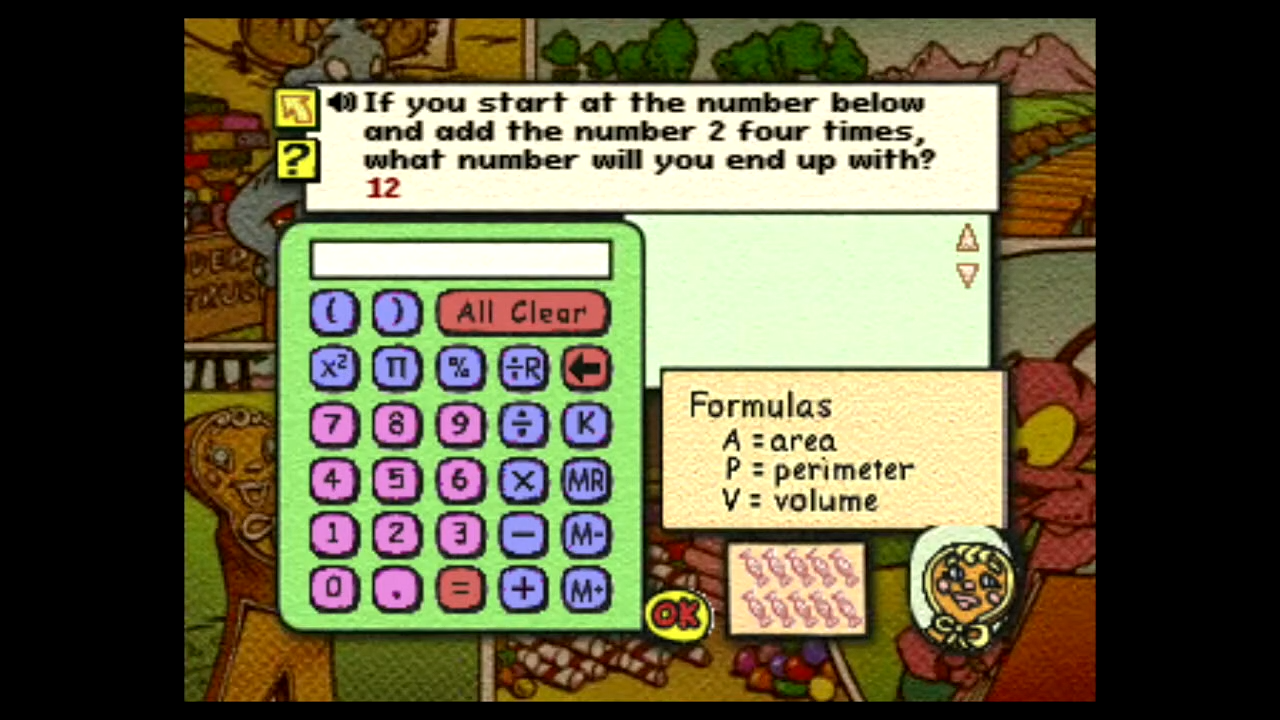
\includegraphics[width=\linewidth]{Games/MathGalleryCollection/Images/MathGalleryCollection1Image4.png}
        \caption{Math Gallery: Collection 1 - Screenshot 4}
    \end{subfigure}
    \caption{Screenshots from Math Gallery: Collection 1}
\end{figure}